\section*{Appendix}
\subsection*{A. Hyperparameter optimization}
\renewcommand{\thefigure}{A\arabic{figure}}
\setcounter{figure}{0}
\renewcommand{\thetable}{A\arabic{table}}
\setcounter{table}{0}

In this appendix we provide the optimal values of the hyperparameters for both the FT-based models and the MULT-based models. Thus, Table A1 shows the hyperparameters of the two different categories of models for each dataset. 

\begin{table}[h]
\caption{Optimal hyperparameters of FT-based and MULT-based models based on SemEval 2015 and SemEval 2016.}
\label{tab:hyperparams}
\setlength{\tabcolsep}{24pt}
\begin{tabular}{@{}lcccc@{}}
\toprule
               & \multicolumn{2}{c}{SemEval 2015} & \multicolumn{2}{c}{SemEval 2016} \\ \cmidrule(l){2-5} 
               & FT              & MULT           & FT              & MULT           \\ \midrule
L1 regulariser & $10^{-9}$           & $10^{-7}$          & $10^{-4}$           & $10^{-5}$          \\
L2 regulariser & 0.000           & 0.001          & 0.000           & 0.000          \\
Learning rate  & 0.001           & 0.001          & 0.001           & 0.001          \\
Dropout rate 1 & 0.3             & 0.3            & 0.5             & 0.6            \\
Dropout rate 2 & 0.4             & 0.6            & 0.6             & 0.5            \\
d   & 400             & 250            & 200             & 400            \\
Lambda         &                 & 0.25           &                 & 0.5            \\ \bottomrule
\end{tabular}
\footnotesize\textit{Note}. Dropout rate 1 refers to the dropout rate at the input layer, while dropout rate 2 refers to the dropout rate after the BiLSTM layer.
\end{table}

\subsection*{B. Confusion matrix and sensitivity analysis}
\renewcommand{\thefigure}{B\arabic{figure}}
\setcounter{figure}{0}
\renewcommand{\thetable}{B\arabic{table}}
\setcounter{table}{0}

Table \ref{tab:confusion matrix:pret} shows the confusion matrix of the PRET+FT model on the SemEval 2015 dataset. The behaviour is similar to the MULT model as discussed in Sect. 5.2, however less pronounced and performance-enhancing.
\begin{table}[h!]
\caption{Confusion matrix of the PRET+FT model with document knowledge transfer for the SemEval 2015 data.}
\label{tab:confusion matrix:pret}
\setlength{\tabcolsep}{28.3pt}
\begin{tabular}{@{}lccc@{}}
\toprule
                   & \multicolumn{3}{c}{Predicted sentiment} \\ \midrule
 Observed sentiment & Negative     & Neutral    & Positive    \\ \midrule
 Negative           & 161          & 4          & 43          \\
 Neutral            & 19           & 4          & 15          \\
 Positive           & 35           & 1          & 318         \\ \bottomrule
 \end{tabular}
 \end{table}
 
 Fig. \ref{fig:pret+ft} shows the model performance for PRET+FT on the SemEval 2015 dataset with varying sizes of the pretraining corpus. The size of the pretraining corpus is step-wise enlarged by 3000. Note that for any of the inspected sizes, the performance does not deteriorate with respect to the LCR-Rot-Hop++ benchmark model, which is equivalent to PRET+FT with a pretraining corpus size of 0. This means that adding domain-relevant documents in the PRET stage will likely not harm the model. Up until 12000 documents, the validation accuracy follows an upwards trend. This suggests that some document knowledge transfers well to the aspect level. However, after its peak at 12000, both the accuracy and macro-F1 seem to jitter. This suggests that too much pretraining data is fed into the model, leading to overfitting on the auxiliary task and underfitting on our main task.
 
 \begin{figure}[h!]
    \centering
    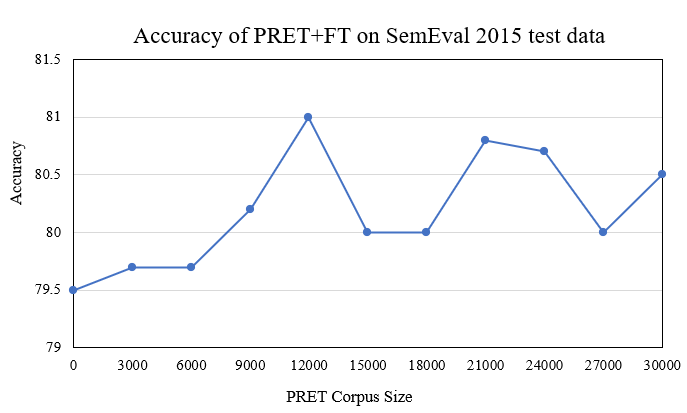
\includegraphics[scale =0.8]{Images/PRET+FT.PNG}
    \caption{Performance of the PRET+FT model for varying pretraining corpus sizes.}
    \label{fig:pret+ft}
\end{figure}